\chapter{Related work}

\section{Provenance Overview}
\label{sec:provenance_overview}

As mentioned above, provenance is historically used in the field of antiques as a guide to authenticity of quality. In this thesis we focus on the more modern concept of digital provenance, a metadata that stores the lienage of a file. Only recently defined, below are two papers outlining the requirements and definition of digital provenance.

\littitle{Carata2014}
\label{sub:a_primer_on_provenance}

Published in the \textit{Communications of the ACM} magazine, this article gives an in depth introduction to digital provenance. It presents current research in the field from a practical perspective and talks at length about their possible use cases as well as issues obtaining, using and securing provenance.

This paper does an impressive job of laying out the fundamentals of digital provenance, as well as identifying current research efforts and areas of improvement. It also describes the language and terminology used by the provenance community when discussing different features of provenance, such as the concepts of \textit{granularity} and \textit{layering} when collecting provenance.

\littitle{Groth2012}
\label{sub:requirements_for_provenance_on_the_web}

This paper from \textit{The International Journal of Digital Curation} synthesizes three main categories that can be used to assess the adequacy of different online provenance systems. It splits these categories into multiple dimensions for finer grained analysis.

The three main categories this paper uses as a base for assessing provenance systems is: content (the data itself and information stored in it), management (different ways of collecting and storing the data) and use (different ways of using the data, visualisation etc.). Each of these categories is then divided into a multitude of related dimensions. For example the \textit{Content} category includes versioning (records of changes written to artefacts over time) and attribution (sources that contributed to making an artefact) as dimensions. The papers support their claims for the requirements of these dimensions by describing them in relation to three scenarios. The scenarios are well picked in order to mirror real world applications.

This paper outlines a range of dimensions that can by used in order to assess an interface. In terms of HCI these can be used as the base for tasks to test on users as well as suggesting features that may be useful in my application. For example, one of the dimensions for \textit{Use} is \textit{Imperfections}, suggesting that I need to take into account that erroneous/imperfect provenance data may exists when creating my interface.

\section{Provenance Acquisition}
\label{sec:provenance_acquisition}

Provenance can be acquired in a variety of ways. A common goal in the literature is to collect provenance automatically and transparently in order to reduce cognitive load on users as well as reducing erroneous or false data. The papers below discuss the collection of provenance across two different layers: operating system level and application level, both with their advantages and disadvantages.

\subsection{OS level provenance acquisition}
\label{sub:os_level_provenance_acquisition}

OS level provenance acquisition stores the calls between different processes and files. It has the advantage of clearly showing what applications rely on which resources and can be used via a custom kernel to log provenance on a computer without requiring any changes to the users applications.
However because of its intrinsic need to treat processes as ``black boxes'' it can also trigger false positives when graphing lineage. For example a process may invoke the use of multiple libraries however it is arguable as to whether they're all relevant in terms of provenance.

\littitlesub{Muniswamy2006}

Published in 2006, the PASS paper is often cited in related literature as a prime example of OS level provenance collection. This paper discusses the advantages of having provenance information maintained by the storage system as well as presenting a PASS implementation with analysis of its performance costs.

In most implementations provenance is stored in a standalone database systems or flat files. This paper argues that provenance should be maintained by the storage system since it is the storage system that manages existing metadata for files. This allows tighter coupling between data and provenance as well as allowing the transparent collection and management of provenance information. The paper lists a set of requirements for a PASS system as well as their own implementation. They benchmarked their implementation on a 500Mhz Pentium 3 computer with 768MB of RAM. The two primary benchmarks used are small and large file microbenchmarks. In the case of the small file benchmark the overhead associated with creating and writing files was as much as 200\%, however its noted that the absolute numbers are still quite small and that this benchmark in particular is quite challenging to PASS. Results from the large file benchmark where better with a time overhead of no more than \%10-\%20.  It seems more reasonable that real users will only encounter overheads of the latter in daily use. Overall the PASS system provides extra functionality not currently available in other systems with only a moderate overhead. It is also important to note that the systems used for these benchmarks are a lot less powerful that what average users use today.

\subsection{Application level provenance acquisition}
\label{sub:application_level_provenance_acquisition}

Application level provenance acquisition has the advantage of creating more relevant relationships between different entities. However it suffers from the overhead required to implement effective capturing and in a lot of cases onus on the user to annotate their actions. Most of the papers below discuss a system that requires developers to somehow modify (usually marginally) their application in order to correctly collect provenance.

\littitlesub{Guo2012}

Authored by Margo Seltzer (one of the top contributors of the field\cite{Macko2012,Seltzer2011,Borkin2013,Muniswamy-Reddy2010,Braun2008},) and Philip J. Guo, this paper presents one of the many ways to collect provenance on a computer. It focuses primarily on research relate provenance and its application in respect to \textit{lab notebooks}.

The application presented in this paper, Burrito, consists of two parts: an extensible platform that automatically captures provenance as well as a set of applications that allow annotations and querying of that data. Stored in a local MongoDB, provenance is captured though GUI window interactions, OS-level capture (like PASS\cite{Muniswamy2006}) and integration with a versioning filesystem. On top of this is a series of plugins that allow provenance to be captured by the following applications: microphone, xpad, Firebox, Chrome, Vim, Bash, Python and the clipboard. Burrito then provides four applications that allow interaction with the provenance data. An activity feed that sits on the users desktop, presenting provenance events chronologically and allowing annotation of events as they happen. A computation context viewer that allows exploration of a files changes and how they impacted output. An activity context viewer that shows what was been read and written at the time of an activity. Finally they also provide a Lab Notebook generator that creates a HTML file summarising the users activities. Over a month this system accumulates approximately 2GB of data and although no benchmarks are reported it is stated to have minimal overhead.

This paper is interesting as it brings provenance to the forefront of the users mind. The goal been that they are constantly annotating and referencing past provenance activities during the length of a project. It also has the added advantage of having images and other program output inline the visualisations.

\littitlesub{Macko2012}

Written in 2012 the authors of this paper Macko and Seltzer are both heavy contributors of the provenance field. Whilst most of the other provenance frameworks mentioned in this review are limited to a particular workflow or language, Macko and Seltzer argue that the real world is a lot more heterogeneous and to accommodate for this they argue the need for a general-purpose provenance library.

This paper presents the Core Provenance Library (CPL) a C++ application that allows the integration of provenance storage into any application. It supports bindings for C, Java and perl as well as a command a line tool for creating shell scripts. The provenance is stored on a database system of your choice through two drivers; these where tested to work for MySQL, PostgreSQl and 4store. The main disadvantage of this framework is that it is the onus of the developers to implement calls to the provenance framework in their application. Multiple features are implemented in order to allow easier integrating such as automatically taking care of persistent storage, cycle detection and resolution, as well as supporting query visualisation through map orbiter~\cite{Seltzer2011}. However developers/project managers need to take into consideration integration when developing an application.

This library provides hope for a standardised way of capturing provenance information. However as mentioned above it is up to developers to correctly integrate it and there's an intrinsic trust that correct and truthful provenance will be recorded. Disappointingly the \href{https://code.google.com/p/core-provenance-library/}{google code repository} hasn't been updated since 2012 and no replacement github repository has been created in light of the shutdown of Google code, suggesting that the project is no longer maintained.

\littitlesub{Allen2010}

This paper describes the ability to compose multiple provenance-unaware services in an ``open world'' system and collect provenance information about their execution. It presents a provenance collection application that sits upon the enterprise service bus (ESB) in order to log provenance information from communicating applications.

This paper advocates for a provenance collection solution that doesn't require system-invasive strategies such as custom kernels or modified applications. It argues that in order to be useful in the ``open world'' provenance capturing tools must fulfil the following tasks, capturing provenance:
\begin{itemize}
  \item across multiple systems with no assumption of control.
  \item from legacy systems
  \item at the level of application interaction, \textit{not} foundational technology stack.
\end{itemize}

In order to evaluate their ESB MULE Capturing Agent (MCA) they tested it upon two different workloads: Loan Borker (a standard MULE test scenario) and CoTLooper (a scenario that uses cursor on target messages). The average time to log provenance within MULE over time decreased as the more provenance nodes where created eventually evening out around $1 \times 10^8ns$. However if message reflection (a method for examining runtime behaviour of applications in the Java VM) was required to gather data from the payload of the message then message capture time can be greatly increased. Whilst these metrics are useful in identifying the overhead of using an ESB to capture provenance information from communicating applications (in this case minimal), itis arguable that the provenance information would suffer from problems similar to OS level capturing systems, creating false positive edges in the graph.

This paper is highly cited in the provenance community. It shows one of the many \textit{layers} of provenance that can be recorded and is one of the few systems that records provenance across multiple machines. 

\section{Provenance Storage}
\label{sec:provenance_storage}

Once provenance has been captured by one of the methods mentioned above, it has to be stored somehow. In a lot of early papers the provenance was stored in different proprietary flat file formats. Since then a standard has been created by the W3C, as well as research into how provenance can be stored on the cloud.

\littitlesub{primer2013}

This online document is an initiative by W3C to create a standard as by which to discuss and store digital provenance. This paper is part of a series of documents outlining different aspects of the PROV standard, in particular it is a primer on the fundamental PROV concepts.

This document outlines the three mains concepts illustrated in Figure~\ref{fig:key-concepts}, as well as different serialisations in languages such as XML, JSON and PROV-N. Each of the concepts are briefly described as:
\begin{itemize}
	\item Entities: Physical, digital, conceptual objects
	\item Activities: Elements that cause an entity to come into existence
	\item Agents: Someone or something that can be assigned responsibility for an actity taking place.  
\end{itemize}

\begin{figure}[h]
	\centering
	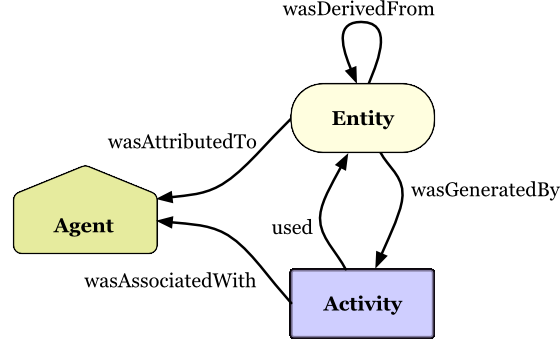
\includegraphics[width=0.5\linewidth]{key-concepts}
	\caption{Key concepts and relationships from the PROV standard displayed in a labelled acyclic graph.}
	\label{fig:key-concepts}
\end{figure}

I used the standards defined in this paper as the oracle definition for provenance in my designs. My prototype was built so that it can read provenance files in the PROV-N format.

\littitle{Muniswamy-Reddy2010}

This paper presents the following problem: although cloud data and provenance both exist, they are not usually used in conjunction because it is difficult to store both in the same location. Traditionally if data is stored in a database, the related provenance information is then stored somewhere else. To mitigate this they present 3 different methods for maintaining data and provenance in current cloud stores.

This paper's contribution is three protocols (using off the shelf software,) each satisfying a different number of properties crucial for provenance systems: provenance data coupling, multi-object casual ordering, data-independent persistence and efficient querying. Each of the systems work with minimal overhead and surprisingly the protocol that fulfils all four of the afore mentioned properties runs as well if not better than the other protocols. The benchmarks used on each of the protocols where varying in their workloads, ranging from CSV backup simulations to workloads representing scientific computation. There is a diverse selection of workloads that simulate scenarios that provenance would most likely be used in.

This creates an avanue of further research. Currently my prototype interface only reads locally stored flat provenance files. In the future it would be useful to expand this to provenance stored on the cloud as well.

\section{Provenance Security}
\label{sec:provenance_security}

Once provenance is captured and stored the issue of securing it is paramount. Simple per-attribute access permissions are ineffective for provenance entities because so much information can be gathered from relationships. It is alos worth considernig how to secure the data in such a way that history can't be ``re-written''. The below papers discuss this problem in greater detail.

\littitle{Braun2008}

A discussion paper from 2008, Margo, Uri and Avraham focus on the issue of properly securing the access rights of provenance data. It frames the problem and identifies issues requiring further research.

This paper aims to start discussion and highlight the importance of considering provenance security during the implementation and development of an application. It proves that provenance cannot be secured in the same way as traditional data because of its ability to provide information through relations as well as the artefacts themselves, arguing instead that provenance needs its own security model. The paper suggests that there is three main aspects of provenance that needs to be secured, each in their own way: the \textit{node data}, the \textit{relationships} between nodes and the \textit{attributes} related to nodes or relationships. It gives concrete examples of why each of these aspects need to be protected and why regular access control methods aren't satisfactory.

This piece is though provoking in the issues it outlines related to securing provenance. It raises the question of how to present partial graphs caused by users with limited permissions. A problem also worth considering in future work is that of how to present to a moderator which bits of a graph are accesible by who.

\littitle{Cheney2011}

A common theme among papers regarding provenance systems is that they agree that provenance is an open and unsolved issue. This paper from the University of Edinburgh outlines a formal model for provenance, formalization of security fundamentals \textit{disclosure} and \textit{obfuscation} and exploration of its implications in various domains.

This paper identifies five main classes of provenance policies: availability, confidentiality, integrity, reverse-engineering and explanation. They go on to describe a high level security framework focusing on the availability (ensuring information about input is available to users) and confidentiality (ensuring that confidential information is never disclosed to a user) of provenance data. This framework is general enough to not be specific to any one system, meaning its rules and obvservations can be applied to any system. The paper provides support to its claims through detailed mathematical proofs. It also provides three instances of how the provenance security framework can be used to create provenance policies.

Unfortunately this paper provides limited benefit to my project because its focus on security is abstract enough to be most useful to researchers designing provenance security systems. However it provides understanding of the security issues involved as well as ideas of how security will be implemented. 

\littitle{Hasan2009}

This paper is often referenced because of it work in creating \textit{Sprov}, a secure provenance storage method. 

The author's main contribution from this paper is \textit{Sprov}, a prototype of the secure provenance primitives, implemented as wrapper functions for the standard I/O library in C. They use a chain encryption method in order to accomplish their primary security goal: stopping undetected rewrites of history. In order to evaluate the Sprov library it was run through a number of benchmarks that simulate different deployment settings. They tested two different configurations for chain storage, both recording straight to disk and also storing on RAM with a chrom daemon periodically flushing the chain to disk. Postmart benchmark was used with a dataset containing 20,000 files ranging in size from 8KB to 64KB. Different write loads where tested all the way from 0-100\%. In its worse case scenario of 100\% writes, Sprov had an overhead of 25\% using disk storage and 11\% using RAM. Small and large file microbenchmarks was used to measure the overhead as a percentage of file size. Interestingly smaller files had a larger overhead, this is thought to be attributed to disk caching (similar results have been found by other provenance benchmarks).

This paper shows one of the many ways provenance data can be used and recorded. Its relevancy to my project is in understanding how provenance will be stored and protected as well as issues that arise in a user interface only showing partial data.

\section{Provenance Display}
\label{sec:provenance_display}

Lastly we come to the field of thesis. How to display provenance. As mentioned previously, provenance never reduces in size, it is forever expanding and been added to. Issues quickly arrise when trying to present such vast amounts of information. The primary issue been that users can't process such large graphs effectively.

\subsection{Visualisation fundamentals}
\label{sub:visualisation_fundamentals}

There's a series of fundamentals that have been tried and tested in the field of visualisation as important rules to follow when developing visualisation tools. Ben Shneiderman discusses fundamental tasks that should be accomplished by visualisation exploration software in order to be effective. A HCI paper then presents how non-technical users view provenance information.

\littitlesub{Shneiderman1996}

Published in 1996 this paper is seen as one of the core papers cited when discussing complex visualisation software. It recommends seven properties that should be implemented by an advanced graphical user interface: overview, zoom, filter, details-on-demand, relate, history and extract. It distils these tasks into what's known as the Visualisation Information Seeking Mantra:

\textit{Overview first, zoom and filter, then details-on-demand}\\
\textit{Overview first, zoom and filter, then details-on-demand}\\
\textit{Overview first, zoom and filter, then details-on-demand}\\
\textit{etc.}

Each of these tasks is explained in great detail with arguments as to why they are necessary. It also provides examples of how different applications have implemented certain tasks, providing an array of examples to research in regard to my project.

I used this paper as a primary starting point when creating my prototype. It was effective as a means of outlining the scope of my application, defining what features where and where not importand.

\littitlesub{Bachour2015}

A Human Centred Technology research project, this paper focuses on collecting feedback from non-expert uses on their understanding of provenance. Through the medium of an online game they explore how well users understand the W3 prov standard\cite{primer2013} and its related artifacts as well as their general opinions and beliefs on provenance data.

The main contributions taken from this paper involved the feedback users gave on the representation of provenance information: one example I found particularly interesting is that a lot of users found the directional arrows confusing. The PROV standard is historical, so directional arrows between nodes are used to represent that something came from something else, however most users found this counter-intuitive and believed that the arrows should have been the other way around to show chronological ordering. The researchers use a game they created based in an Orwellian future in order to explain the concept of provenance. Users were presented with provenance graphs that they had to identify mistakes in. Eight players agreed to hour-long phone interviews and 41 submitted online questionnaires. Although the use of an online game as a usability study is unconventional its merits are well argued in the paper as well as citing other research papers that have used similar methods.

This paper provides some useful feedback from non-technical users as to what issues they perceive when dealing with provenance graphs and allows me to start my interface designs with preliminary user feedback. In conjunction to heuristic feedback the paper also provides some insight into non-expert users opinions on the security/privacy issues of provenance as well as their understanding of its real world applications.

\subsection{General Large Graph Visualisation}
\label{sub:large_graph_visualisation}

Effective large graph visualisation is an on open issue in many fields outside of provenance. Both of the visualisation techniques presented below use a clustering mechanism for grouping relevant nodes. 

\littitlesub{Abello2006}

This paper presents an interface for exploring large-scale graphs. The visualisation tool is generic in so far as its made for the exploration of graphs in general. It uses a clustered graph to represent information with the ability to arbitrarily expand and collapse clusters to show sub-graphs.

The paper focuses on creating an interface that can present large-scale graphs to users without been impeded by system performance. This paper goes into quite some depth relating to the algorithms used to cluster nodes as well as methods used to maintain usability with constrained resources (although it is important to note that this was written in 2006 and the issue of constrained resources may not be as relevant today). It also explores issues related to naming clusters: the authors decide on a tag based labelling system that they state is sub-optimal for understanding the contents of a cluster. No formal usability study was undertaken, the authors note that the application was in continuous use by data analysts over the six months preceding publication. It is promising that preliminary feedback was collected in this time (such as users wanting to annotate sections of the graph) and implemented into the application.

This paper's main relation to my research includes the problems tackled when visualising such large graphs. Design decisions related to clustering and pre-processing provided to be useful in creating my interface as well as issues presented in labelling clusters. 

\littitlesub{Schaffer1996}

With this paper been nearly twenty years old its obvious how much younger the provenance research field is in comparison to visualisation. This paper talks about using a novel fish-eye interface in order to show large graphs while allowing users to zoom into particular nodes and not lose context. They also provide usability study results in order to support their claim that fisheye views improve performance compared to traditional variable-zoom interfaces.

This paper sets out to research the problems created by viewing large-scale graphs in a variable zoom interface. The authors create a usability test in order to compare the time taken to complete certain tasks on two interfaces. The first is a variable-zoom interface that allows the user to control the zoom level of the entire graph and pan around to find information. The other is a fisheye interface that clusters nodes and allows expansion of clusters in order to view greater detail. The subjects where asked to act as telephone technicians and had to navigate a network graph in order to identify a broken telephone line as well as rerouting lines in order to `repair' the network. The main metric for identifying interface effectiveness was time (in seconds) taken to complete tasks. Using the fisheye interface users on average completed the task 60 seconds faster than when using the variable-zoom interface. Although not statistically analysed the authors also noted that nearly one third of fish-eye results showed a near optimal route when rerouting, whilst variable-zoom results didn't come close to being optimal.

This paper raises some interesting points about the importance of allowing users to have `peripheral vision' when browsing large complex graphs. There is useful details about how they chose to scale magnified clusters as well as discussion about how to accommodate overlapping clusters. Interestingly they run into similar issues as \cite{Abello2006} when trying to label clusters, except 10 years earlier.  

\subsection{Provenance display tools}

There is a diverse range of existing provenance display tools that aim to present provenance to users in an easy to understand way. Whilst most of the applications use a directed acyclic graph to present provenance information, there is also representation through the use of Sankey diagrams and orbital graphs, which depending on what information you wish to portray can sometimes be more effective than DAGs.

\littitlesub{Seltzer2011}

As provenance data becomes more common, the amount of provenance information continues to expand. It is not uncommon for the size of provenance data to greatly outweigh its target file, creating provenance data that has upwards of thousands to millions of nodes. This paper presents a Java application that can be used to visualise large scale provenance graphs through the use of zooming and summation techniques.

This paper's core contribution is a cross-platform Java application, titled ``Map Orbiter'', that can be used to visualise RDF/N3 and OPM formatted provenance data. It simplifies complex graphs by grouping related nodes into \textit{summary nodes} and allows users to view more information about a summary node by \textit{zooming} in. It also supports the filter task, allowing users to pick a subsetof nodes that they would like to view. 

This application is often referenced in other provenance visualisation papers as the primary example of directed acyclic graph visualisation. It focuses on similar issues to my project, but focuses on a Java implementation and reads provenance in the RDF/N3 and OPM format.

\begin{figure}[h]
	\centering
	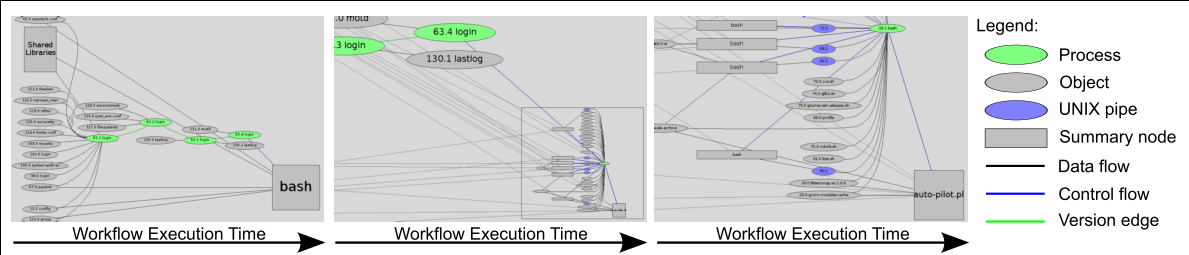
\includegraphics[width=\linewidth]{maporbiter}
	\caption{A screenshot of Mab Orbiter and its semantic zoom. Left: a high-level view of Linux’s login process and its dependencies. Middle \& Right: the progress of zooming into the bash summary node (in the lower-right corner), representing the login shell and the corresponding user session.}
	\label{fig:maporbiter}
\end{figure}

\littitlesub{Biton2007}

This paper is a demonstration that shows how user views can be used to reduce the amount of information returned by provenance queries. It allows users to select which parts of a provenance graph (referred to in this paper as a \textit{work flow}) they find relevant and have the original graph simplified to only include the parts they picked, as seen in Figure~\ref{fig:zoomuserviews}

Similar to clustering, the ZOOM interface simplifies parts of a provenance graph by collapsing nodes, however instead of creating a cluster object, ZOOM creates a replacement \textit{composite} node. The paper illustrates how it generates provenance information from logs stored on an Oracle warehouse as well as outlining some of the optimisations that can be used in Oracle 10.2 to aid in the generation of immediate provenance. The authors also discuss what properties they believe important when collapsing nodes into composites, what features make a ``good'' user view. These features include preserving the inputs and outputs from relevant nodes and hiding as much detail about irrelevant nodes as possible. In terms of size the examples in this paper are limited to graphs of 19 nodes, although extensions for larger graphs are foreseeable through extensions of the application.

This interface is similar to what I ended up designing and implementing. The primary differences are that my application uses provenance files from the PROV-N standard and that my application is designed for provenance exploration, whilst the ZOOM*UserViews system is aimed at simplifying graphs for use by other people.

\begin{figure}[h]
	\centering
	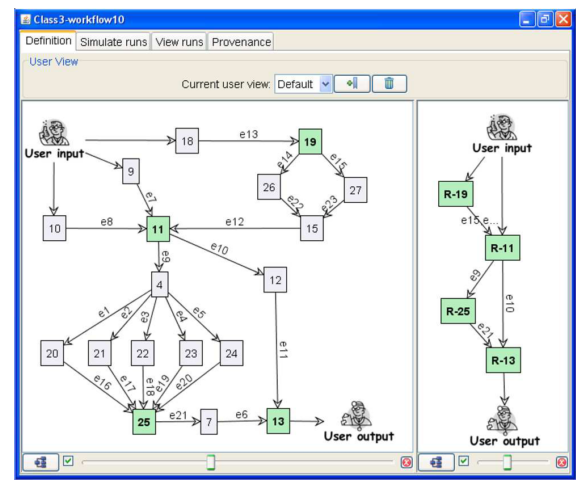
\includegraphics[width=0.8\linewidth]{zoomuserviews}
	\caption{A Screenshot of the Zoom*UserViews application. On the left is the entire provenance graph with parts selected and on the right is the simplified graph created from the selected parts.}
	\label{fig:zoomuserviews}
\end{figure}


\littitlesub{Hoekstra2014}

This paper presents an application called PRO-O-Vis that uses Sankey Diagrams in order to reflect the flow of information through activities. It discusses the application, reasoning behind representation through Sankey diagrams and a brief evaluation of their application.

This papers main contribution is an online tool that can be used to view provenance information stored in the PROV-O format. Once provenance has been uploaded it generates a viewer that allows exploration of the provenance by selecting an activity to focus on (from a dropdown menu) and presenting its related Sankey diagram. The interface is entirely web based and can be embedded in other websites completely self contained (doesn't require API calls to a server). A brief evaluation of the application has been made using four different sources and issues were found regarding input that had a large number or related activities, this could sometimes cause a delay in generating multiple Sankey diagrams. The paper briefly argues the use of Sankey diagrams over DAG graphs as they more easily allow visualisation of magnitude of flow within a network, comparatively complex DAG graphs can make it hard to view this information.

This application differs from other visualisation tools in the field as it's implemented completely in web tools whilst many of the visualizers run on Java. Because of this it is one of the easiest visualisation tools to install and get running because you mearly have to use a web browser. I used this as inspiration for implementing my prototype as a web application. 

\begin{figure}[h]
	\centering
	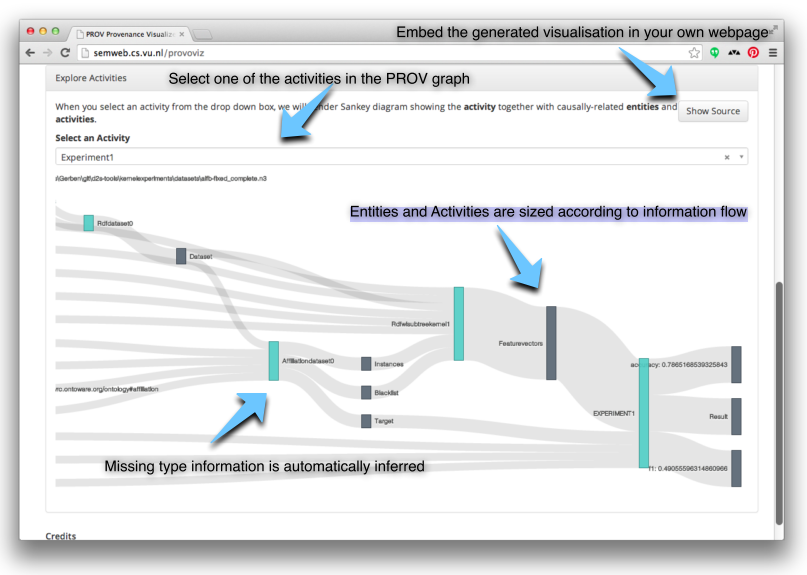
\includegraphics[width=0.8\linewidth]{provovis}
\caption{Overview report of a runtime experiment, generated by the Prov-O-Vis system.}
	\label{fig:provovis}
\end{figure}

\littitlesub{Callahan2006}

This is one of the earlier papers mentioning the concept of provenance as we know it today. Published at SIGMOD in 2006, this paper discusses the importance of provenance in generating visualizations. It presents an application called VisTrails that can be used to create visualizations whilst recording provenance during exploration to aid in later scrutiny and replication.

This paper states that existing visualization tools are limited because they do not record the provenance of their outputs. VisTrails improves on the downfalls of existing visualization tools through the use of provenance. This paper was written before any provenance standards~\cite{Macko2012} so the application instead stores all relevant provenance information in an XML formatted file. The application uses provenance in order to record \textit{evolving dataflows}, (where a dataflow is a form of visualization pipeline) allowing the modification of existing dataflows in order to compare and contrast resulting visualisations. Because provenance is captured related to changes to dataflows, it's possible at any point to check the history of a particular dataflow and identify what modifications where made to get to its current state. The VisTrails system was demonstrated through 3 examples although no references are made to any current real life uses of the application.

This paper is interesting as it's one of the earliest papers I've found in my research that identifies the importance of provenance. Its example of using provenance for visualization replication also shows how adaptable provenance can be to different scenarios, particularly its usefulness in exploratory situations. Its an important paper in order to be able to understand how the concept of provenance evolved into its current form.

\begin{figure}[h]
	\centering
	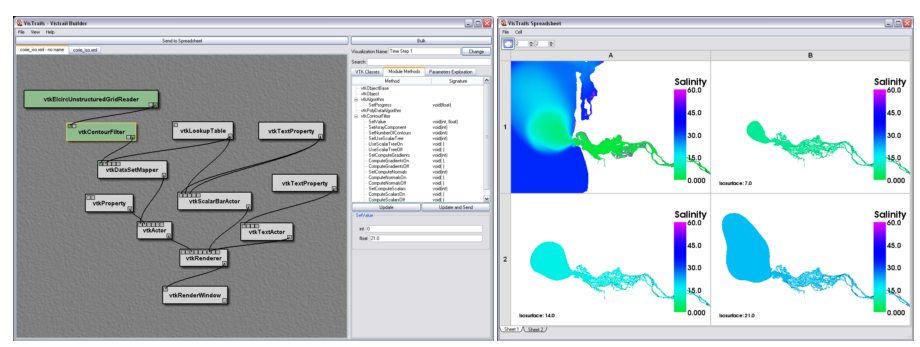
\includegraphics[width=0.9\linewidth]{vistrails}
	\caption{A screenshot of the VisTrails system. On the left you can see the provenance of a figure from a report. On the right is different versions of that figure that have been created.}
	\label{fig:vistrails}
\end{figure}

\littitlesub{Borkin2013}

This paper focuses on the visualisation of provenance information relating to filesystem: the read and writes between processes and files. The authors implement a visualization tool called InProv and both qualitatively and quantitatively compare it's effectiveness to one of the standard provenance visualisation tools Orbiter\cite{Seltzer2011}.

This papers main contributions are: Firstly, qualitative research with domain experts in order to create a set of requirements for a provenance visualiser. Secondly, InProv a provenance visualization tool that uses a radial layout and chronological clustering. Thirdly, a quantitative user study comparing the effectiveness of the two interfaces InProv and Orbiter. The qualitative research was undertaking via semi-structured one hour long interviews. They asked the domain experts to talk about how they used provenance information as well as demonstrating their daily workflows. Using results from the qualitative research they created a set of core tasks they wished to accomplish and used radial visualisation to create the InProv tool. The user study had 27 participants who where asked to accomplish tasks of varying difficulty on both the InProv and Orbiter interfaces. The metrics used to analyse performance where seconds required to complete task as well as percentage of correctly completed tasks. In most cases the difference between time to complete tasks was not significantly different between the two interfaces. However using a new clustering algorithm that clusters nodes based on time of activity (compared to process tree clustering) was shown to have significant improvement on task completion time by as much as 90 seconds.

This paper provides a lot of useful quantitative and qualitative information through its well laid out user studies. Of most interest is the interviews with domain experts. Also the choice of using \textit{time based hierarchical grouping} is of particular interest because of the large impact it had upon improving usability. This paper makes the largest attempt at conducting a usability study and my tasks were influenced by the tasks the use in this paper.

\begin{figure}[h]
	\centering
	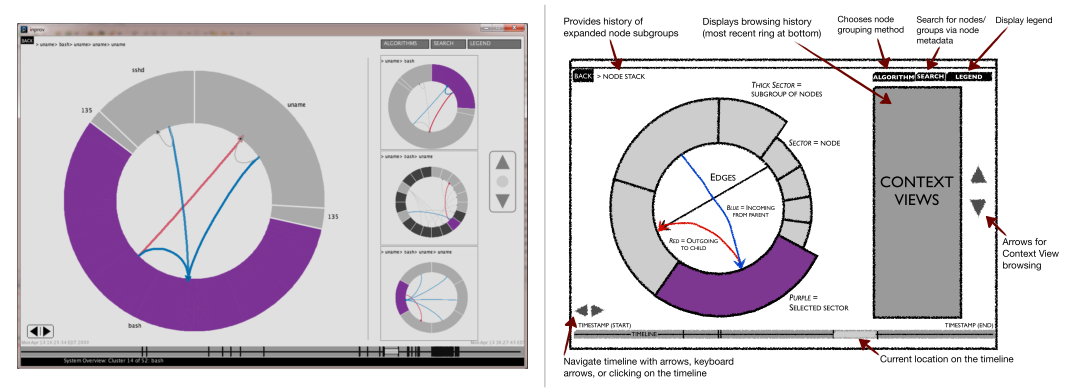
\includegraphics[width=0.8\linewidth]{filesystem}
	\caption{A screenshot and mockup of the InProv visualisation interface using radial diagrams.}
	\label{fig:filesystem}
\end{figure}
